\begin{columns}[totalwidth=.9\linewidth]
    \column{\textwidth}
        \begin{boxnote}
            \textbf{高分子材料でマルチマテリアル化 $\Leftrightarrow$ 高い比強度の有効利用}
            \begin{itemize}
                \item {\color{red} 「接着接合」}への高分子の利用
                    \begin{itemize}
                        \item 柔らかさを生かした{\color{red} 「弾性接着接合」}
                        \item 耐久性、可逆性に優れた\alert{ゴム材料に注目}
                    \end{itemize}
                \item {\color{blue}耐久性が不明確}
                    \begin{itemize}
                        \item 特に疲労破壊に対して
                    \end{itemize}
            \end{itemize}
        \end{boxnote}
\end{columns}

\begin{columns}[totalwidth=.9\linewidth]
    \column{\textwidth}
    \begin{itembox}[l]{ヒステリシスと破壊靭性}
        \begin{columns}[totalwidth=\linewidth]
            \column{.8\textwidth}
                \begin{itemize}
                    \item 力学的ヒステリシス
                    \begin{itemize}
                        \item
                        印荷時に比べて、除荷時の応力が低下する減少
                        \item
                        ヒステリシスロス:変形時のエネルギー散逸
                    \end{itemize}
                    \item 破壊靭性との関係
                    \begin{itemize}
                        \item
                        Andrews 理論:ヒステリシスロスの重要性が指摘
                    \end{itemize}
                \end{itemize}
            \column{.2\textwidth}
                \centering
                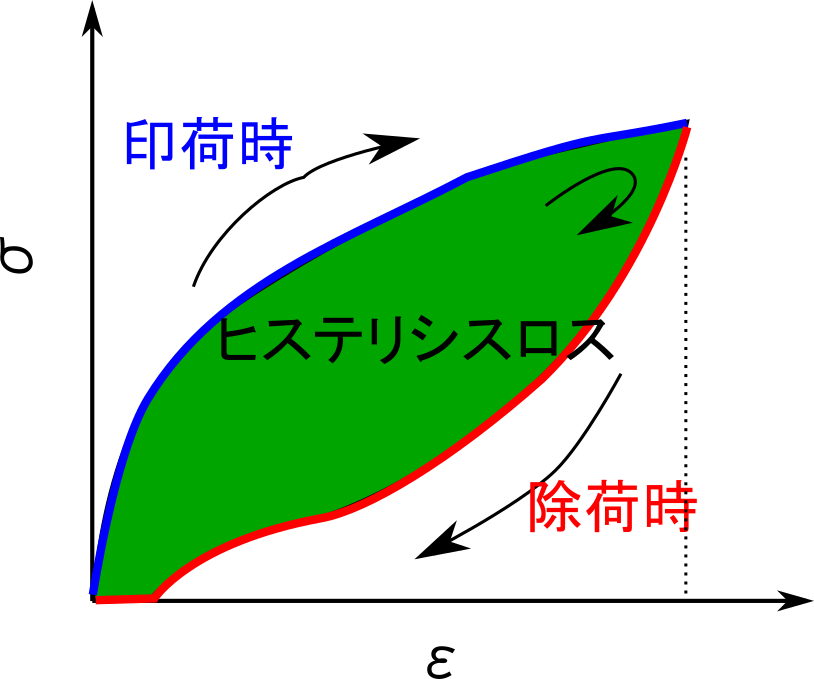
\includegraphics[width=\textwidth]{hysteresis_curve.png}
            \end{columns}
    \end{itembox}
\end{columns}

\begin{columns}[totalwidth=.9\linewidth]
    \column{\textwidth}
    \begin{itembox}[l]{Andrews 理論\cite{andrews}}
        \begin{columns}[totalwidth=\textwidth]
            \column{.8\textwidth}
                クラックの微小進展時に、
                \begin{itemize}
                    \item
                    \textcolor{red}{Loading 場}と\textcolor{blue}{Unloading 場}のひずみエネルギーの差
                    \item
                    全体の変形に要したエネルギーの多くを\textcolor{red}{散逸}
                    \item
                    鎖の破断へのエネルギーが低減 $\Rightarrow$ \alert{強靭さの起源。}
                \end{itemize}	
            \column{.2\textwidth}
                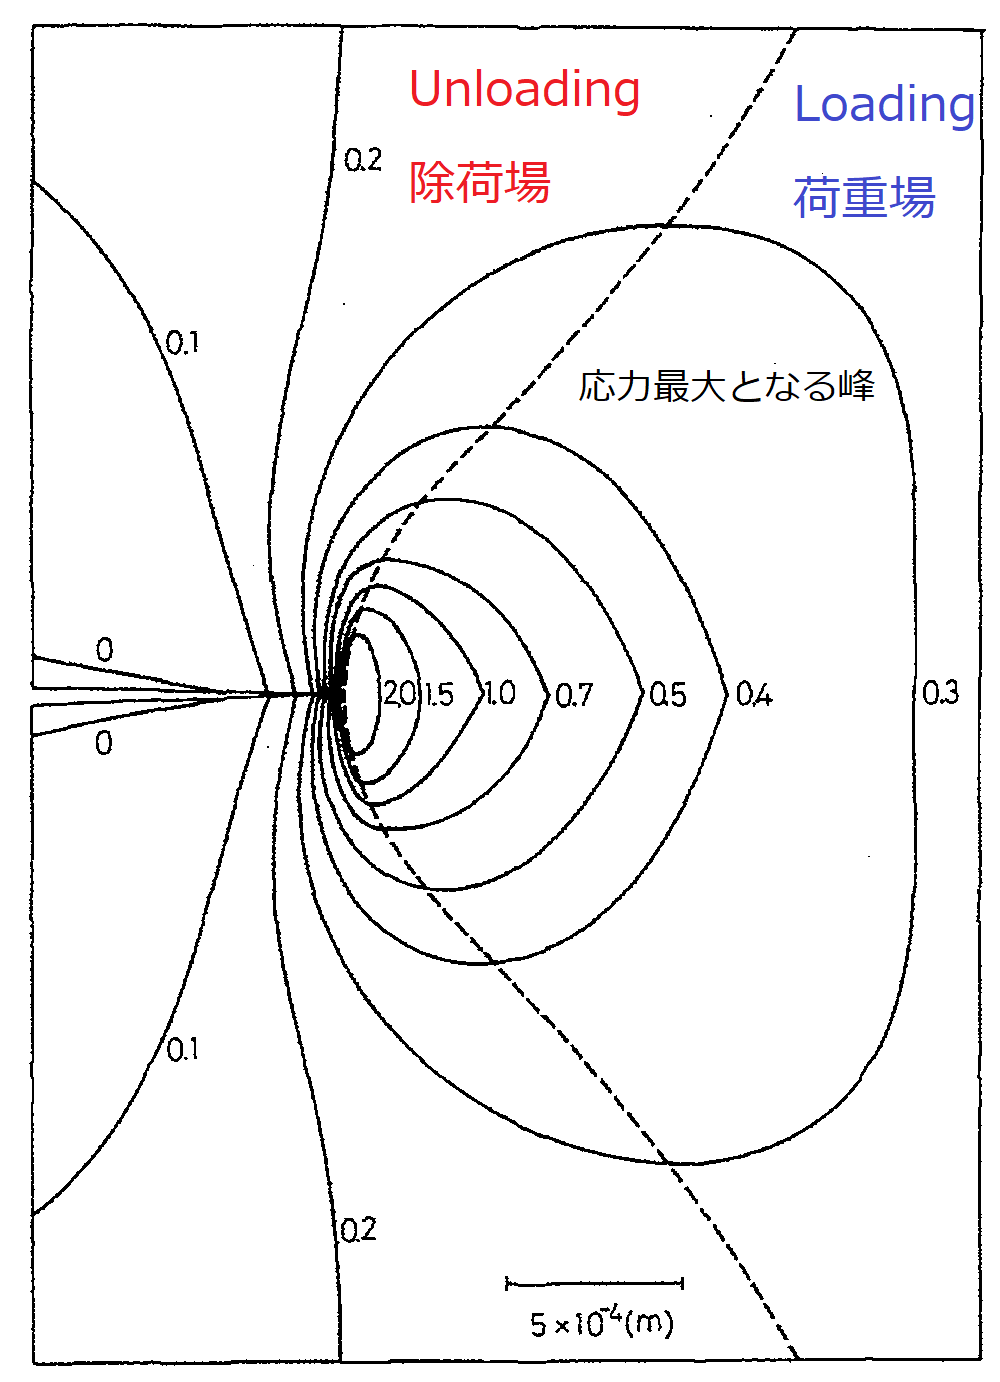
\includegraphics[width=.8\textwidth]{crack.png}     
        \end{columns}
    \end{itembox}
\end{columns}

\begin{columns}[totalwidth=.9\linewidth]
    \column{\textwidth}
    \begin{itembox}[l]{架橋点の環境とランダムな接続性}
        \begin{columns}[totalwidth=\textwidth]
			\column{.3\textwidth}
                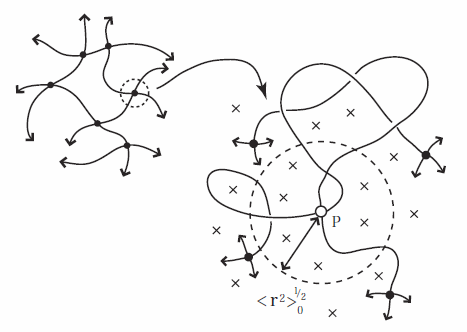
\includegraphics[width=\textwidth]{JP_vicinity.png}
                架橋点は、\alert{多数のストランド(図中の×)}に囲まれている。
			\column{.4\textwidth}
                \begin{itemize}
                    \item 接続性を不均一に
                        % \begin{itemize}
                        %     \item 接続に\alert{位置依存性}
                        % \end{itemize}
                    \item 巨視的な変形後
                        \begin{itemize}
                            \item \alert{結節点のゆらぎが不均一}
                            \item 多様な緩和モード
                            % \item \alert{緩和の長時間化?}
                        \item ファントムネットワークの\\諸特性が発現
                        \end{itemize}
                \end{itemize}
            \column{.3\textwidth}
				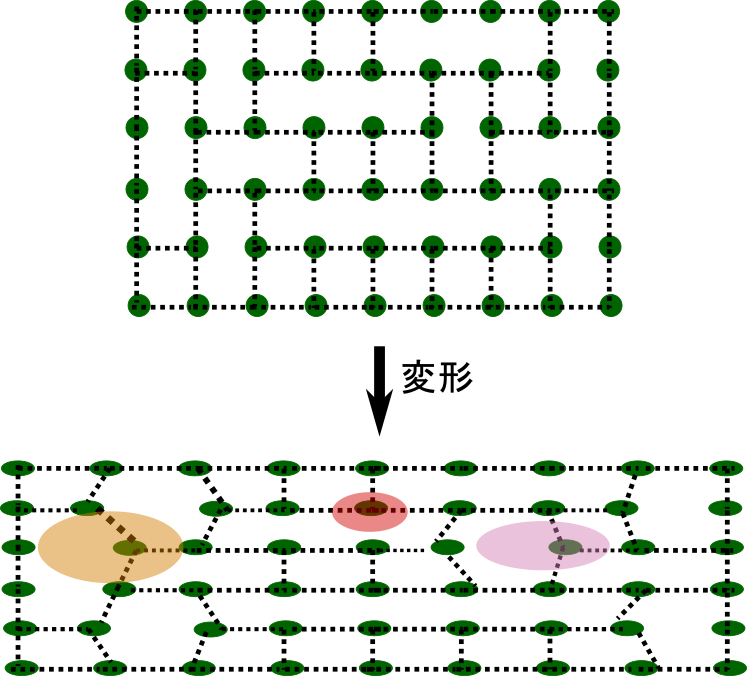
\includegraphics[width=.8\textwidth]{random_NW.png}
		\end{columns}
    \end{itembox}
\end{columns}